% !Mode:: "TeX:UTF-8"
\chapter{基础原理概述}
\label{chap:第二章}
本章主要介绍基于本地知识库的大模型智能反馈交互系统的理论基础,深入分析了大模型基本原理和检索增强生成,包括transformer模型和提示词的理论。此外,模型压缩作为系统的一部分,也被一并阐述。这些理论介绍旨在为后续章节中提出的系统设计提供必要的知识背景。
\section{生成式自回归神经网络}
大模型推理作为检索增强生成的核心功能,依赖于大模型优秀的理解和推理能力,常见的大模型结构有GPT类\cite{floridiGPT3ItsNature2020}和LLaMA\cite{touvronLLaMAOpenEfficient2023}类等。以上两类大模型都属于生成式自回归网络,是一类基于条件概率的模型,即递归地预测下一个单词或符号生成输出。例如,给定输出输入${x_1},{x_2}, \ldots ,{x_t}$,模型会预测下一个生成符号(token)的概率$P({x_{t + 1}}|{x_1},{x_2}, \ldots ,{x_t})$,进而根据分词器生成整个词表的概率分布,得到下一个输出${x_t}$。下面介绍生成式自回归模型的整个输入输出流程即各部分结构及作用。
\begin{table}[!htb]
  \centering
  \begin{minipage}[t]{0.8\linewidth}
    \bicaption[GPT 分词器参数意义]{GPT 分词器参数意义}[content of GPT tokenizer parameters]{content of GPT tokenizer parameters}
    \label{tab:gpt-tokenizer-parameters}
    \begin{tabularx}{\linewidth}{lXl}
      \toprule[1.5pt]
      {\heiti 参数}  & {\heiti 意义} & {\heiti 取值} \\\midrule[1pt]
      词表大小 & 分词器中包含的所有 Token 的总类数 & 50257 \\
      最大序列长度 & 模型支持的最大 Token 序列长度 & 2048 \\
      特殊符号 & 模型中预定义的特殊 Token,用于标记序列的起点、终点或其他特定功能 & [EOS]、[PAD]、[SEP] 等 \\
      填充方式 & 是否对输入序列进行填充 & True \\
      截断策略 & 是否对超过最大长度的输入序列进行截断 & True \\
      \bottomrule[1.5pt]
    \end{tabularx}
  \end{minipage}
\end{table}

首先需要使用分词器(Tokenizer)将自然语言编码成代表其编号的数字,这一过程由两部分组成。分词器首先将文本转化为token,例如将“我是分词器”,转化为[“我”,“是”,“分”,“词”,“器”];再根据训练好的分词表{“我”:101,“是”:2,“分”:80,“词”:890,“器”:568},将分词后的token编码成数字序列[101,2,80,890,568]。以GPT模型的英文分词器为例介绍几种重要参数规格,如表\ref{tab:gpt-tokenizer-parameters}所示。其中特殊符号作用是标记文本中的结构,如起点、终点以及填充符号。填充和截断的作用是当输入文本长度与分词器的输入长度不同时,是否将多余或不足的位置截断或使用填充符号填充。同理,模型最后的输出的数字序列也需要分词器反向查表转化成自然语言,可以方便地将这种操作近似理解成双向的哈希表。

分词器输出的数字序列还需要嵌入模型(Embedding model)转化成向量才能作为模型的输入。嵌入模型将一维的数字序列转化成高维的词向量,词向量维度根据大模型的规模不同而不同,如LLaMA-7B的参数量为70万(Billion),嵌入维度为4096,LLaMA-65B的参数维度为8092。现在主流的嵌入模型都是基于transformer\cite{devlinBertPretrainingDeep2018}模型训练的,其结构与大模型主要结构相似,将和下面大模型结构统一介绍。

最早提出的生成式模型为transformer\cite{vaswaniAttentionAllYou2017}模型,由编码器和解码器两部分组成,而每部分都是由transformer块串联构成,如图\ref{fig:transformer}。在transformer块中,使大模型具有高性能的关键就是注意力机制(attention)。注意力机制的核心思想是让模型能够根据输入数据的不同部分分配不同的权重,从而更高效地处理信息。注意力机制通过计算查询向量(Query)、键向量(Key)和值向量(Value)之间的关系,生成一个权重分布,然后用这些权重对值向量(Value)加权求和,得到输出。
\begin{equation}
  \label{eq:attention}
  Attention(Q,K,V) = \text{softmax}\left(\frac{QK^T}{\sqrt{d_k}}\right)V
\end{equation}
其中$Q$、$K$、$V$由输入嵌入向量和系数矩阵计算得到,$d_k$为$K$向量的维度,用于缩放防止数值过大。$softmax(\cdot )$定义为,
\begin{equation}
  \label{eq:softmax}
  softmax({z_i}) = \frac{{{e^{{z_i}}}}}{{\sum {_{j = 1}^n{e^{{z_j}}}} }},{\rm{  }}i = 1,2,...,n
\end{equation}
将输出结果转化为概率分布。模型结构中也使用了线性层和残差链接\cite{heDeepResidualLearning2016}改善模型性能。

与原始的transformer模型不同,生成式自回归模型采用encoder-only(decoder-only)结构,根据历史输出产生新的输出,如图\ref{fig:encodel}所示。上文中提到的嵌入层也是encoder-only结构,与图\ref{fig:encodel}不同的是最后的输出线性层,具体结构同bert\cite{devlinBertPretrainingDeep2018}。Encoder-only模型每次推理只产生一个token的概率分布,要想生成一个完整的句子需要根据前文多次推理,也就是自回归。所以需要特定的生成规则,选择每次生成的哪个token。ChatGPT 模型的生成机制由解码策略、上下文限制和停止条件等核心规则共同构成。解码策略决定了模型如何从概率分布中选择输出标记,包括常见的方式如贪心搜索\cite{bahdanauNeuralMachineTranslation2016}、束搜索\cite{sutskeverSequenceSequenceLearning2014}、随机采样\cite{radfordImprovingLanguageUnderstanding2018}、Top-k\cite{fanHierarchicalNeuralStory2018} 采样和Top-p(核采样)\cite{holtzmanCuriousCaseNeural2020}策略。这些策略在生成质量和多样性之间平衡,适用于不同场景。例如,贪心搜索计算高效但容易陷入局部最优,Top-p 采样则通过动态调整候选范围提高多样性。
\begin{figure}[htbp]
  \centering
  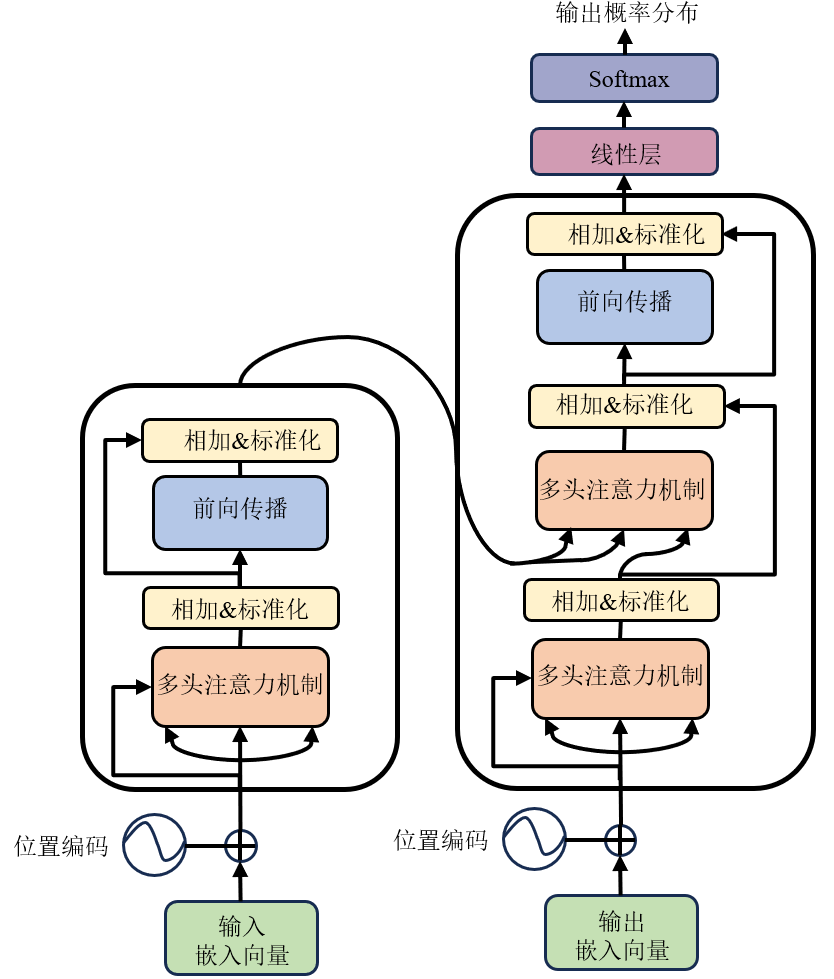
\includegraphics[scale=0.44]{transformer结构.png}
  \bicaption[transformer结构]{transformer结构}[]{ Transformer Structure}
  \label{fig:transformer}
\end{figure}
\begin{figure}[!htbp]
  \centering
  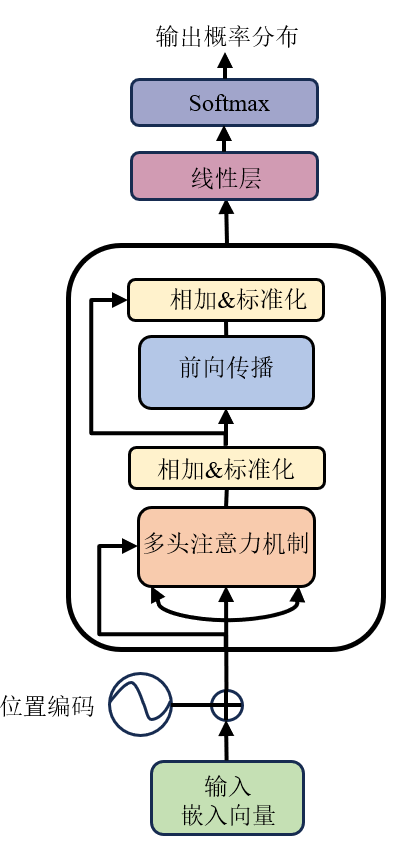
\includegraphics[scale=0.44]{encoderonly.png}
  \bicaption[encoder-only结构]{Encoder-only结构}[]{ Encoder-only Structure}
  \label{fig:encodel}
\end{figure}


\section{提示词学习}
提示词学习(Prompt Learning)是一种新的模型优化方法,通过设计输入格式或附加提示(prompts),使语言模型更好地理解任务意图并生成符合期望的输出。与传统微调(Fine-tuning)方法不同,提示词学习通常不需要修改模型参数,而是通过输入结构的调整激发模型内部的知识,从而完成特定任务。
\subsection{提示词学习理论基础}
提示词学习最早的雏形是由OpenAI在验证GPT-2模型能在无监督(zero-shot)的情况下学习语义与任务知识\cite{radfordLanguageModelsAre2019}。GPT-2模型在参数上达到了1542M,已经通过预训练学习了大量通用知识及理解能力,不需要再通过额外样本学习来完成任务,但仍需要通过一些方法令模型理解任务需求,输出符合预期的结果,如图\ref{fig:监督学习示意图}。图中以二分类情感分析任务为例,适当调整模型的输出层以适应任务后,通过大量的训练样本令模型学习语义知识并告诉模型面对不同的输入该对应什么结果,并将这种行为更新在模型参数中。因此,再次得到相似的输入时就可以得到正确输出。
\begin{figure}[!htbp]
  \centering
  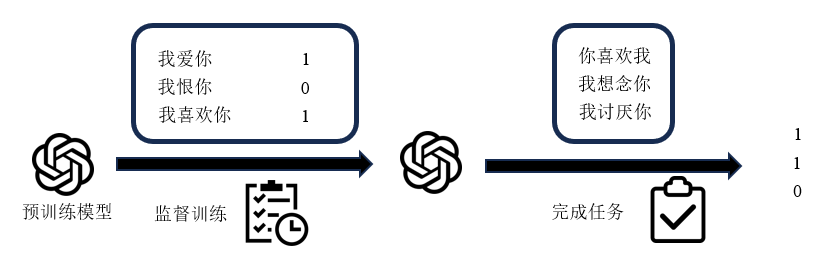
\includegraphics[scale=0.55]{监督训练示意图.png}
  \bicaption[监督学习示意图]{监督学习示意图}[Supervised Sraining]{Supervised Sraining}
  \label{fig:监督学习示意图}
\end{figure}

而面对大规模参数的预训练模型GPT-2时,研究人员认为通过大量的文本预训练以及百万参数量级的参数已经令模型具备足够的理解能力和通用知识,所以只需要简单的少样本(Few-shot)微调来使模型熟悉输入输出模式即可。但因为模型参数庞大,即使少量样本的训练也需要大量的运算资源,并且在特定任务下难以获取足够高质量样本,研究者们逐渐探索不需要特定任务数据下的零样本(zero-shot)方法来使预训练模型完成下游任务,即早期提示词学习的雏形。

在这种方法中,不对模型的参数进行更新而是对下游任务数据进行预处理,将文本嵌入进数据集中,通过文字的方式让模型理解任务的需求,同时规范化输出格式,如图\ref{fig: 零样本学习示意图}所示。
\begin{figure}[!htbp]
  \centering
  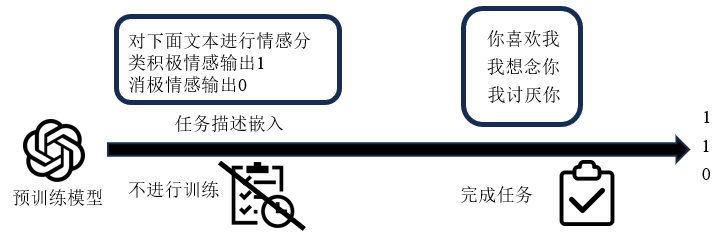
\includegraphics[scale=0.57]{零样本学习示意图.png}
  \bicaption[零样本学习示意图]{零样本学习示意图}[]{Zero-shot Learning}
  \label{fig: 零样本学习示意图}
\end{figure}

实验表明,这种只做文本嵌入不做特定训练框架的方法在多个自然语言处理任务中达到了最优结果,部分任务中远超基线模型。作者证明,具有足够容量的语言模型可以通过无监督学习执行多种任务,并在部分任务中达到或超过 SOTA (State of the Art)性能。这一发现为多任务学习和预训练语言模型的发展提供了重要的思路。即通过在数据中加入描述性文本来替代下游任务训练的无监督学习方法。

\subsection{提示词学习方法}

本节中介绍在实际应用中常用到的提示词学习方法,同时也是在检索增强系统中实际应用的方法,以便理解提示词在系统中的原理及意义。
少样本(Few-shot)学习是在零样本学习后提出的,根据零样本学习的研究成果,作者相信更大参数规模的模型配合上适量训练数据可以更进一步地提高模型在复杂下游任务上的表现,而训练数据也是作为提示词的形式输入给模型,不需要训练来更新参数就可以规范化模型的输出格式,如图\ref{fig: 少样本学习提示词样例}。图中展示了针对表格问答任务的输入输出样例。通过少量的样例就可以令模型理解任务,并且直接通过样例让模型理解任务需求的方式比直接通过语言描述任务需求效果更好更直观,还可以规范生成式模型的回答格式。以上方法为检索增强生成的核心原理,研究人员将之定义为离散提示词学习。
\begin{figure}[htbp]
  \centering
  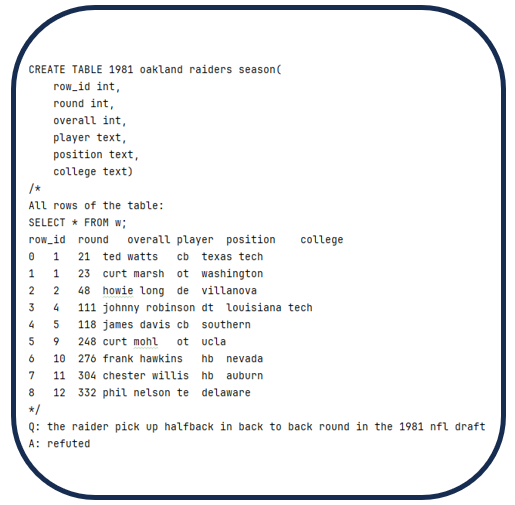
\includegraphics[scale=0.74]{少样本学习提示词样例.png}
  \bicaption[少样本学习提示词样例]{少样本学习提示词样例}[]{Few-Shot Learning Prompt Example}
  \label{fig: 少样本学习提示词样例}
\end{figure}


\section{神经网络模型压缩}
循环神经网络(Recurrent Neural Network,RNN)是一类在处理序列数据方面具有独特优势的神经网络,广泛应用于自然语言处理、时间序列分析等众多领域。其设计初衷是为了有效处理数据中的时间序列信息或序列依赖关系。从结构角度来看,RNN 区别于传统神经网络的核心特征是其具有反馈连接。在 RNN 的架构中,隐藏层既接收当前时刻输入层的信号,又会整合上一时刻隐藏层自身的输出信息。这一特性使得 RNN 能够在处理序列数据时,保留并利用先前时间步的信息,进而捕捉数据中的长期依赖关系。在$t$时刻的RNN单元可以表示为
\begin{equation}
  \label{eq:rnn}
  {h_t} = \varphi ({W_{xh}}{x_t} + {W_{hh}}{h_{t - 1}} + b)
\end{equation}
其中,$x_t$表示时刻t的输入向量,$h_{t-1}$是上一时刻$t-1$的隐藏层状态向量,$h_t$则为当前时刻的隐藏层状态向量;$W_{xh}$和$W_{hh}$分别是输入到隐藏层和隐藏层到隐藏层的权重矩阵,它们决定了不同输入对隐藏层状态的影响程度;$b$是偏置向量,用于增加模型的灵活性;$\varphi$代表激活函数,如常见的$sigmoid$函数、$tanh$ 函数等,其作用是对加权输入进行非线性变换,使模型能够学习到复杂的非线性关系。为方便与文章后续内容比较和理解循环神经网络与非线性动力学系统之间的联系将循环神经网络表示为公式\ref{eq:rnn2}。
\begin{equation}
  \label{eq:rnn2}
  {x_t} = f(A{x_{t - 1}} + B{u_t})
\end{equation}
其中$x_t$为当前t时刻的隐藏层状态,$A$为隐藏层到隐藏层的状态系数矩阵,$B$为输入到隐藏层的输入稀疏矩阵,$u_t$为当前时刻t的输入,$f()$表示激活函数。下面介绍动力学系统(dynamical system)及其非线性的内容及表达形式。

动力学系统是一门融合数学、物理学及工程学等多学科理论,专注于研究随时间演化的系统行为的学科领域。它通过建立数学模型,对系统状态随时间的变化规律进行精确刻画,揭示系统的内在动态特性,为众多科学与工程问题提供理论依据和解决方案。这里主要介绍离散非线性动力学系统,非线性动力学系统是动力学系统的一个重要分支,它聚焦于研究随时间演化的系统,且系统内各元素之间存在非线性相互作用关系。相较于线性系统,非线性动力学系统能够展现出更为丰富和复杂的行为,这些行为无法通过线性理论进行全面解释与预测从数学定义上看,非线性离散动力学系统通常由一组非线性差分方程来描述,如公式\ref{eq:discrete}。
\begin{equation}
  \label{eq:discrete}
  {x_k} = g({x_{k - 1}},{u_k},k)
\end{equation}
其中$x_k$为当前离散时刻$k$的状态,$u_k$为当前离散时刻$k$的输入,$g()$代表任意函数映射关系,当$g()$为非线性函数时,系统即为非线性离散动力学系统。通过表达系统内部各个状态于采样时间之间的映射关系来描述系统模型,并通过数学方法分析和处理系统。循环神经网络于动力学系统模型的具体关系将在第\ref{cha:第三章}章中详细介绍。

降维(Dimensionality Reduction)作为解决高维数据与复杂系统建模问题的核心思想,在神经网络模型压缩与动力学系统模型降阶中均占据重要地位。尽管二者分属机器学习与动力系统领域,但其方法论在降维思想上具有深刻的一致性,均通过对高维空间的结构化近似与稀疏化表示,实现模型复杂度的降低与计算效率的提升。神经网络模型压缩通过减少参数量与计算复杂度来优化模型性能,而动力学系统模型降阶则通过简化复杂微分方程描述的动态过程来降低数值求解的复杂度。二者的核心目标均是在保留关键特征的前提下,将高维空间映射至低维空间,从而实现高效建模与计算。

在神经网络模型压缩中,降维思想主要体现在参数剪枝\cite{liuFilterPruningQuantifying2023}、量化\cite{jacobQuantizationTrainingNeural2018}、知识蒸馏\cite{hintonDistillingKnowledgeNeural2015}以及低秩分解\cite{hanDeepCompressionCompressing2016}等方法中。参数剪枝通过移除冗余权重实现模型的稀疏化表示,其本质是对高维参数空间的降维操作,利用显著性准则(如权重幅值或梯度敏感度)识别并裁剪非关键连接,从而将稠密参数矩阵转化为稀疏矩阵。量化则通过将高精度浮点参数映射至低比特整数表示,实现参数空间的降维,极端情况下,二值化网络将权重约束为±1,将高维连续空间映射至低维离散空间。知识蒸馏利用教师网络的软标签指导轻量化学生网络的训练,本质上是将教师网络的高维特征空间压缩至学生网络的低维空间,通过提取教师网络的关键特征,学生网络能够在低维空间中近似原始模型的性能。低秩分解通过将权重矩阵分解为多个低秩矩阵的乘积,显著减少参数量,例如奇异值分解法(SVD)
\begin{equation}
  \label{eq:svd}
  W_n = U_n\Sigma_n {V_n^T}
\end{equation}
\begin{equation}
  \label{eq:Sigma}
{\Sigma_n} = \begin{array}{*{20}{c}}
  {{\sigma _1}}&0& \cdots &0\\
  0&{{\sigma _2}}& \cdots &0\\
   \vdots & \cdots & \cdots & \vdots \\
  0&0& \cdots &{{\sigma _n}}
  \end{array}
\end{equation}
其中$U_n$、$\Sigma_n$、$V_n$分别为权重矩阵$W_n$的左奇异值矩阵、奇异值矩阵与右奇异值矩阵,$\sigma_i$为矩阵$W_n$的奇异值,并按非递增顺序排列。通过保留主要奇异值与对应奇异值向量,实现权重矩阵的降维。将权重矩阵分解为奇异向量与奇异值的组合,或两个矩阵的乘积形式,从而减少参数量,
\begin{equation}
  \label{eq:lowrank}
  W_n \approx {\hat{U}_{n\times m}}{\hat{V}_{m\times n}^T}
\end{equation}
其中,$m(m<n)$为保留的奇异值个数,$\hat{U}$、$\hat{V}$分别为保留前$m$个向量的左奇异值矩阵和奇异值矩阵与右奇异值矩阵的乘积$\hat{V}=\Sigma_mV$,通过适当选择$m$,可以有效压缩参数量,保留主要奇异值以实现降维。这些方法在卷积神经网络中广泛应用,也是大模型的低秩近似轻量化微调(adapter)\cite{houlsbyParameterefficientTransferLearning2019}的主要理论方法,能够有效降低计算复杂度。

在动力学系统模型降阶中,降维思想则通过投影降阶、平衡截断、时间尺度分离以及非线性降维等技术实现。投影降阶通过基函数投影将高维状态空间映射至低维子空间,例如本征正交分解(POD)提取主成分构成降维基,将高维动力学系统嵌入到低维子空间中,从而保留系统的主要动态特征。平衡截断基于可控性与可观性Gram矩阵,剔除对输入-输出行为贡献微弱的状态变量,其本质是通过对状态空间的压缩,保留系统的主导动态行为。时间尺度分离通过奇异扰动理论将多速率系统的快慢变量分离,仅保留慢变子系统,利用系统动态特性的时间尺度差异,将高维动力学系统降维为低维慢变系统。

尽管神经网络模型压缩与动力学系统模型降阶在应用场景上存在差异,但二者的降维思想在数学本质与方法论上具有高度一致性。首先,二者均依赖于低维嵌入与稀疏表示的思想,模型压缩中的剪枝与量化可视为对参数空间的稀疏约束,而动力学降阶通过投影消除冗余状态变量,二者均利用稀疏性先验实现降维。其次,二者的优化目标具有同构性,均需最小化简化模型与原始模型的误差,例如知识蒸馏的损失函数与POD中的主成分保留均体现为对关键特征的提取与保留。此外,二者的方法论在某种程度上相互借鉴与融合,例如平衡截断中的Hankel范数优化思想可迁移至神经网络,通过分析权重矩阵的奇异值分布指导分层剪枝;而自编码器结构被引入非线性系统降阶,其编码器可视为数据驱动的POD基生成器,实现了从数据中自动提取低维特征。
然而,二者也存在一定差异。神经网络模型压缩侧重静态参数空间的优化,通常依赖数据驱动的方法;而动力学系统模型降阶则关注动态演化过程的近似,通常基于物理方程的先验知识。这种差异使得二者在具体实现上有所不同,但也为二者的协同提供了可能性。例如,在实时控制系统中,压缩后的轻量化网络可作为降阶模型的替代,实现嵌入式部署;而动力学降阶技术可为网络训练提供更高效的计算方法,提升训练效率。

\begin{table}[htb]
  \centering
  \begin{minipage}[t]{0.8\linewidth}
    \bicaption[模型压缩和模型降阶比较]{模型压缩和模型降阶比较}[Comparison of Model Compression and Model Reduction]{Comparison of Model Compression and Model Reduction}
    \label{tab:model-compression-reduction}
    \begin{tabularx}{\linewidth}{lXX}
      \toprule[1.5pt]
      {\heiti 参数} & {\heiti 模型压缩} & {\heiti 模型降阶} \\\midrule[1pt]
      定义 & 通过减少模型参数量与计算复杂度,保持性能 & 通过简化微分方程描述的动态过程,保留系统主要动态特征 \\
      数学本质 & 参数空间的稀疏约束与低维嵌入 & 状态空间的降维与简化 \\
      数据依赖性 & 依赖数据驱动 & 基于物理方程的先验知识 \\
      目的 & 平衡模型复杂度与精度,实现轻量化部署 & 保留系统主要动态行为,简化数值求解 \\
      主要技术 & 剪枝、量化、知识蒸馏、低秩分解 & 投影降阶、平衡截断、时间尺度分离、非线性降维 \\
      \bottomrule[1.5pt]
    \end{tabularx}
  \end{minipage}
\end{table}

神经网络模型压缩与动力学系统模型降阶在方法论上虽属于机器学习与动态系统领域,但其核心思想均以降维理论为基础,旨在通过低维嵌入与稀疏表示实现高维复杂系统的简化建模。二者在数学本质上具有显著共性:均需构造误差泛函以最小化简化模型与原始模型的特征偏差(如模型压缩的预测误差与降阶系统的动态响应误差),并依赖稀疏性约束(如参数剪枝与投影降阶)提取关键特征。然而,其差异主要体现在优化对象与应用层面:模型压缩聚焦于静态参数空间的轻量化(如权重矩阵的量化与低秩分解),依赖数据驱动方法优化边缘计算场景下的推理效率;模型降阶则针对动态演化过程(如微分方程状态变量的时间尺度分离),基于物理先验知识保留系统的可控性与可观性模态。此外,二者的理论基础亦存在差异——前者基于流形(flow)近似理论重构参数空间,后者则依托理论提取动态模态。尽管如此,两类方法在实时控制、嵌入式系统等交叉场景中展现出协同潜力,例如通过物理约束增强网络泛化性,或利用轻量化网络替代传统降阶模型,为跨领域的高效建模提供了新的理论框架。

循环神经网络(RNN)在连续提示词学习中的编码作用主要体现在其对时序动态特征的有效捕捉与上下文信息的渐进式建模。连续提示词\cite{liuPTuningV2Prompt2022}是在寻找最优离散提示词的基础上提出的,希望通过一段无实际含义但可训练的向量来代替离散的词向量,以实现最优的提示词效果。在连续提示词中最重要的是连续提示词向量的初始化嵌入,嵌入模型既要考虑编码的轻量性又要包含语序信息。RNN作为一种经典的序列模型,具有较好的时序建模能力,能够有效捕捉提示词序列中的长程依赖关系,成为了实现该功能的首选工具。
RNN通过其循环结构逐时间步处理连续提示词的序列输入,并通过隐藏状态传递历史信息。以长短期记忆网络(LSTM)为例,其门控机制(输入门、遗忘门、输出门)可自适应调节提示词序列中不同时间步的权重,从而区分关键提示与冗余噪声。例如,在对话生成任务中,LSTM可将用户输入的连续提示词(如上下文意图向量)编码为固定维度的隐藏状态,作为解码器的初始化上下文,确保生成文本的语义连贯性。此外,RNN通过迭代更新隐藏状态,实现对多层级提示特征的融合。在连续提示学习中,初始提示(如任务描述向量)与动态补充提示(如检索增强的上下文向量)可通过RNN的时序编码进行层次化整合。例如,在文本分类任务中,双向GRU(门控循环单元)可将任务相关的连续提示词与输入文本的嵌入向量按时间顺序融合,生成上下文敏感的特征表示,提升模型对复杂语义边界的判别能力。

相比于Transformer等自注意力模型,RNN的计算复杂度与序列长度呈线性关系,更适合资源受限场景下的连续提示学习。通过参数共享与增量式处理,RNN能够以较低内存开销支持实时动态提示调整。在低资源机器翻译任务中,基于LSTM的连续提示编码器可将推理延迟降低,同时保持良好的效果。然而,RNN在长程依赖建模能力上存在局限性,未来研究可通过引入记忆增强机制或混合架构(RNN-Transformer协同编码)提升对长提示序列的建模效果。此外,基于可微分结构的动态提示剪枝技术可进一步优化RNN编码效率,实现关键提示特征的精准提取。RNN通过其固有的时序建模能力,在连续提示词学习中实现了对动态提示特征的渐进式编码与上下文感知融合,为轻量化、实时性要求高的任务提供了高效解决方案,未来结合记忆增强与混合架构的设计有望突破其长序列建模瓶颈,推动提示学习的进一步发展。
\section{检索增强生成}
检索增强生成(Retrieval-Augmented Generation, RAG)\cite{karpukhinDensePassageRetrieval2020,izacardFewshotLearningRetrieval2022,yaoEditingLargeLanguage2023,fengTrendsIntegrationKnowledge2023,xuRetrievalMeetsLong2024,balaguerRAGVsFinetuning2024}是一种将外部知识库动态集成到生成模型中的技术方法,其核心目标是通过引入结构化检索机制增强生成内容的准确性、逻辑性与事实一致性。与传统端到端生成模型依赖内部参数化知识不同,RAG系统通过“检索-推理-生成”的协同机制,将生成过程与外部知识库实时交互,有效解决了模型幻觉(Hallucination)与长尾知识覆盖不足等问题。该技术的实现依赖于三个核心组件:检索器(Retriever)、向量知识库(Vector Knowledge Base)与智能协调体(Agent),并通过思维链(Chain of Thought, CoT)的渐进式推理框架实现复杂任务的分解与求解。

在科学问答任务中,传统模型在处理跨学科知识的复杂问题时,常因模型参数偏差导致错误传播,影响答案准确性。而结合思维链(CoT)机制的RAG系统则有效克服了这一局限。
当用户提出涉及多学科知识交叉的复杂问题时,RAG系统首先通过检索器从大规模向量知识库中精准提取与问题高度相关的文档片段。这些片段可能来自不同学科领域,为后续推理提供了知识支撑。接着,系统基于这些检索到的内容,构建出多步推理路径的上下文。这一过程模拟了人类专家在面对复杂问题时的渐进式思维模式,将不同来源的知识有机整合,形成连贯的推理链条。
最后,系统依据构建好的推理链上下文,生成逻辑连贯、内容完整的答案。整个过程通过引入外部知识约束,有效降低了传统模型因参数偏差导致的错误传播风险。

检索器作为连接生成模块与知识库的核心枢纽,其性能直接决定了知识检索的精度与效率。当前主流方法主要分为稀疏检索与密集检索两类:稀疏检索器,基于词频统计构建查询与文档的匹配关系,具有计算效率高的优势,但对语义相似性的捕捉能力有限。典型代表为BM25\cite{robertsonProbabilisticRelevanceFramework2009}算法,通过将目标文本$Query$分词为单个token $q_i$后,再分别计算$q_i$对于某一文本$d$的相似度加权和,如公式\ref{eq:bm25}
\begin{equation}
  \label{eq:bm25}
  \text{score}(q, d) = \sum_{i} W_i \cdot R(q_i, d)
  \end{equation}
其中$W_i$为$q_i$的权重,$R(q_i, d)$为$q_i$与$d$的相似度函数。相似度函数$R()$一般使用余弦相似度计算。
\begin{equation}
  \text{similarity} = \cos(\theta) = \frac{\mathbf{A} \cdot \mathbf{B}}{\|\mathbf{A}\|\|\mathbf{B}\|} = \frac{\sum_{i=1}^{n} a_i \times b_i}{\sqrt{\sum_{i=1}^{n} (a_i)^2} \times \sqrt{\sum_{i=1}^{n} (b_i)^2}}.
  \end{equation}
其中$\mathbf{A}$、$\mathbf{B}$代表需要计算相似度的两个高维向量,$a_i$、$b_i$为对应向量的每个维度上的分量。
密集检索器(如基于BERT、DPR的深度模型)通过神经网络将文本映射为高维稠密向量,利用向量空间相似度实现语义级检索,能够识别查询与文档间的隐含关联,但需依赖大规模训练数据与计算资源。为平衡效率与精度,混合检索架构(如ColBERT模型)通过上下文感知的多向量表示方法,对文档不同片段进行细粒度匹配,在长文本检索场景中表现出显著优势。与此同时,向量知识库的构建与管理面临数据标准化、嵌入编码优化与动态更新等挑战。当前研究通过分块策略(Chunking)与实体链接技术实现非结构化文本的预处理,采用Sentence-BERT等预训练模型生成文档嵌入,并借助FAISS等最邻近算法(Approximate Nearest Neighbor,ANN)等近似最近邻算法建立高效索引。

智能体(Agent)作为RAG系统的控制中枢,负责动态调控检索与生成模块的交互策略。其核心功能包括检索触发决策、多轮检索优化与结果融合策略。例如,当输入问题涉及常识性知识时,Agent可直接调用模型内部参数化知识生成答案;而对于专业性较强的查询,则触发外部检索流程获取补充信息。在生成过程中,若检测到中间推理结果的置信度不足,Agent可发起多轮检索以迭代补充证据。为实现多源检索结果的融合,系统常采用注意力机制对相关片段进行加权聚合,或通过最大内积搜索(MIPS)筛选最相关段落。在技术实现上,智能体多基于强化学习框架构建,通过策略梯度方法优化决策过程,其目标函数同时考虑答案准确性、检索效率与资源消耗等多维度指标。

尽管RAG技术在知识密集型任务中展现出巨大潜力,其实际应用仍面临多重挑战。首先,密集检索与多轮推理导致的系统延迟问题亟待解决,轻量级检索架构(如基于知识蒸馏的检索器压缩)与硬件加速技术成为研究热点。其次,静态向量知识库难以适应动态演化的外部知识环境,如何实现流式数据下的在线嵌入更新与知识修正仍需深入探索。此外,当前RAG系统主要面向文本模态,如何融合图像、视频等多模态知识以支持跨媒体推理成为重要发展方向。未来研究可聚焦于构建端到端可微的联合训练框架,通过检索与生成模块的参数共享提升系统整体效率;开发基于因果推理的检索验证机制,增强生成结果的可解释性;同时拓展RAG在科学发现、法律咨询等垂直领域的应用边界,推动知识驱动型人工智能的实用化进程。
\section{本章小结}
本章系统阐述了基于大模型的智能反馈交互系统的核心理论基础,为后续系统的设计提供了理论支撑与方法论框架。首先,通过分析生成式自回归神经网络(如GPT、LLaMA等)的架构特性,揭示了其通过自回归机制实现序列生成的内在原理,并重点讨论了Transformer模型中的注意力机制与分词器对语义建模的关键作用。其次,从零样本学习到少样本学习的演进路径出发,剖析了提示词学习(Prompt Learning)通过输入任务指令与非参数化知识提高模型下游任务表现的核心逻辑,为检索增强生成(RAG)系统的动态知识整合提供了方法论基础。

在模型压缩理论部分,通过对比神经网络模型压缩与动力学系统模型降阶的数学本质,提出二者均以降维思想为核心,分别通过参数稀疏化与状态空间投影实现高效压缩。特别地,针对循环神经网络(RNN)在连续提示词编码中的文本嵌入能力,分析了其在轻量化推理中的独特优势,为后续基于本征正交分解的模型压缩方法提供了理论依据。  

最后,聚焦检索增强生成(RAG)技术,系统阐释了其“检索-推理-生成”协同的工作机理,强调了检索器、向量知识库与智能协调体的协同优化策略。通过对比稀疏检索与密集检索的技术差异,以及知识库动态更新的实现路径,揭示了RAG系统在知识密集型任务中的核心价值。本章内容不仅为后续章节的模型压缩算法设计、表格推理框架构建及反馈系统实现奠定了理论基础,更通过跨学科视角(如动力学系统与深度学习的融合)为轻量化智能系统的开发提供了创新性研究方向。


